\documentclass{article}
\usepackage[utf8]{inputenc}
\usepackage{float}
\usepackage{graphicx}
\usepackage{hyperref}
\usepackage{cleveref}
\usepackage{xcolor}
\usepackage{subcaption}
\usepackage{listings}
\usepackage{tabularx}
\hypersetup{
    colorlinks,
    linkcolor={black!50!black},
    citecolor={blue!50!black},
    urlcolor={blue!80!black}
}
% Default fixed font does not support bold face
\DeclareFixedFont{\ttb}{T1}{txtt}{bx}{n}{8} % for bold
\DeclareFixedFont{\ttm}{T1}{txtt}{m}{n}{8}  % for normal
\usepackage{color}
\definecolor{deepblue}{rgb}{0,0,0.5}
\definecolor{deepred}{rgb}{0.6,0,0}
\definecolor{deepgreen}{rgb}{0,0.5,0}

% Python style for highlighting
\newcommand\pythonstyle{\lstset{
language=Python,
basicstyle=\ttm,
otherkeywords={self},             % Add keywords here
keywordstyle=\ttb\color{deepblue},
emph={MyClass,__init__},          % Custom highlighting
emphstyle=\ttb\color{deepred},    % Custom highlighting style
stringstyle=\color{deepgreen},
frame=tb,                         % Any extra options here
showstringspaces=false            % 
}}
% Python environment
\lstnewenvironment{python}[1][]
{
\pythonstyle
\lstset{#1}
}
{}

% Python for external files
\newcommand\pythonexternal[2][]{{
\pythonstyle
\lstinputlisting[#1]{#2}}}

% Python for inline
\newcommand\pythoninline[1]{{\pythonstyle\lstinline!#1!}}



\title{Visualizing fakenews as reported by euvsdisinfo.eu}
\author{Jesper Henrichsen \\{\small Supervised by: Pedro Ferreira}}
\begin{document}
\maketitle
\newpage
\tableofcontents
\newpage

%%%%
% Some title section: A visualization of fake news reported by euvsdisinfo.eu
%%%%
\section{Introduction}
Since the introduction of the internet, information has been able to reach further and faster than ever before. Recent developments of omnipresent social media has created the perfect platform for the spread of this information within the internet. For the sake of advertisement social media platforms has, since their introduction, only become better at targeting their audience with information that will capture their attention. As put by the team behind the newsfeed at Facebook: ``{\it The goal of News Feed is to deliver the right content to the right people at the right time (...)}''. However, a relevant question would be to whom it is implied to be {\it right} for. That it is not necessarily the user, has recently emerged as a likely answer.   
% That the answer is not necessarily the user, has emerged as the likely 
% In the wake of the latest right swing in western  has emerged as the likely answer 
%However, the context is important to understand the consequence of this statement when the main purpose is to generate money through advertisement. Then, the statement comes to mean something alike whatever information will get the user to interact with the content, and in that equation, the quality of the actual content becomes irrelevant. 
% Then, the statement becomes something alike: the information that will get the user to interact with the content, and the equation becomes invariant to the quality of the information. 
\\\\
% Because of the nature of social media, it has proved an effective way to spread misinformation.
The nature of social media, has proved to be an effective way for the spread of information, genuine as well as misinformation.
This report will describe the process of scraping and visualizing information from \href{https://euvsdisinfo.eu}{euvsdisinfo.eu}. One objective was to investigate whether these cases could be used to view fakenews as attacks. And if so, could there be identified a perpetrator either an outlet or country, and a victim as in the country being mentioned in the information.
% \section{method}
\\\\
%%%%% ALTERNATE DRAFT:
% With most people using social media as their main source of information, targeted internet advertisement has proved to be the perfect storm for internet trolls, government agencies, and selfconcerned demagogues. The economist suggests that either humour or rage based posts are the most effective vessels for the spread of information on social media. The fact is, that most people will look to share content in a bid to make themselves appear to the world in a certain light.
% Echo chambers are created by the business model of social media firms, with clusters of other users that they are more similar with than with users in other clusters. The similarity measure is based on the likelihood of the users to interact with different types of content. The clusters are so finely tuned that one experiment don by researchers (?) showed that it was possible for anyone to infringe on any particular persons privacy and follow their geographical whereabouts via targeted ads for as little as \$1000 and a delay of only a couple of minutes. However, the clusters for targeted advertisement also optimizes the efficiency of information spread in terms of number of disposed users and the impact (?) as never before. This efficiency coupled with such information being misinformation, fake news, is possibly the greatest threat to democracy of our time. The fact that this tendency to use social media for spreading fake news exploits a conflict of interest for social media firms, for whom it is naive, and in some ways unfair, to expect them to be able to act as a governing body when one such interest is the core pillar of its business model - generate profit for shareholders. For a publiclly traded company, such interest always weighs the most, and any societal concerns will, if need be, come second (Noam Chomsky?). Therefore, in order to combat this great challenge for people to be able to discuss, debate, and reach compromises on the same empirical basis, there needs to be more regulation in this are, however new it may be. The fact taht so many individuals depends and uses social media as their main outlet makes it a concern not just for the individual, but for the society as a whole. Though, in order to make effective regulation, we need better understanding of a phenomena that in many regards are still new. \\\\

\section{Background}
Since 2015 the campaign \href{https://www.euvsdisinfo.eu}{euvsdisinfo.eu}, has been run by the European External Action Service East Stratcom Task Force. The primary focus of the campaign is to identify and debunk pro-Kremlin disinformation.  %According to the 
The campaign includes cases of debunked information from sources spanning from official news sites to twitter accounts, to non-online content such as interviews. The website \href{https://www.euvsdisinfo.eu}{euvsdisinfo.eu} includes, at the time of writing, more than 3400 such cases, these are the cases that this report is based on. The cases are all reported either by the campaign staff themselves, or one of the 400 collaborating organizations and individuals.
In \Cref{fig:cases} is seen how cases are listed on the website, the order of which is chronological with respect to the date it was reported.

\begin{figure}[H]
    \centering
    % \begin{subfigure}[b]{.3\textwidth}
    \caption{Example listing of disinformation cases on \href{https://www.euvsdisinfo.eu}{euvsdisinfo.eu}}
    \label{fig:cases}
    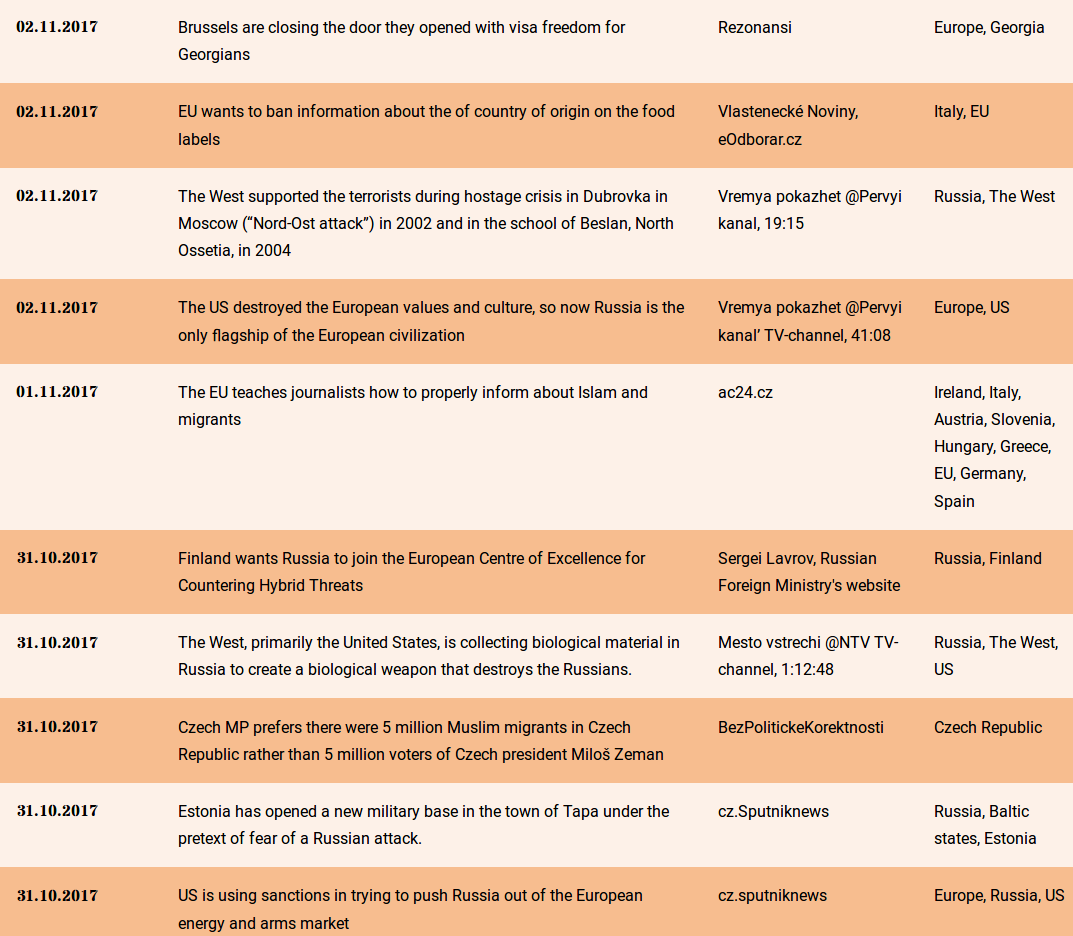
\includegraphics[width=.9\textwidth]{images/example_cases.png}
    % \end{subfigure}%
\end{figure}

\section{Acquiring a dataset}
In this section, the approach to acquiring and extracting information for the visualization will be described. The initial dataset was scraped from \href{https://www.euvsdisinfo.eu}{euvsdisinfo.eu}, however, this dataset was gradually extended in a number of steps. These steps will be described in this section.

\subsection{Scraping the cases}
The cases listed at \href{https://www.euvsdisinfo.eu}{euvsdisinfo.eu} consists of information regarding the case, such as who reported it, in what country or countries did it originate in, as well as the disproof that debunks the information as invalid. Other information for each case is meta information about the information and its source. In \Cref{fig:single_case} is seen an example of the information listed for a specific case.
\begin{figure}[H]
    % \begin{subfigure}[b]{.3\textwidth}
    \centering
    \caption{An example of the information for each case}
    \label{fig:single_case}
    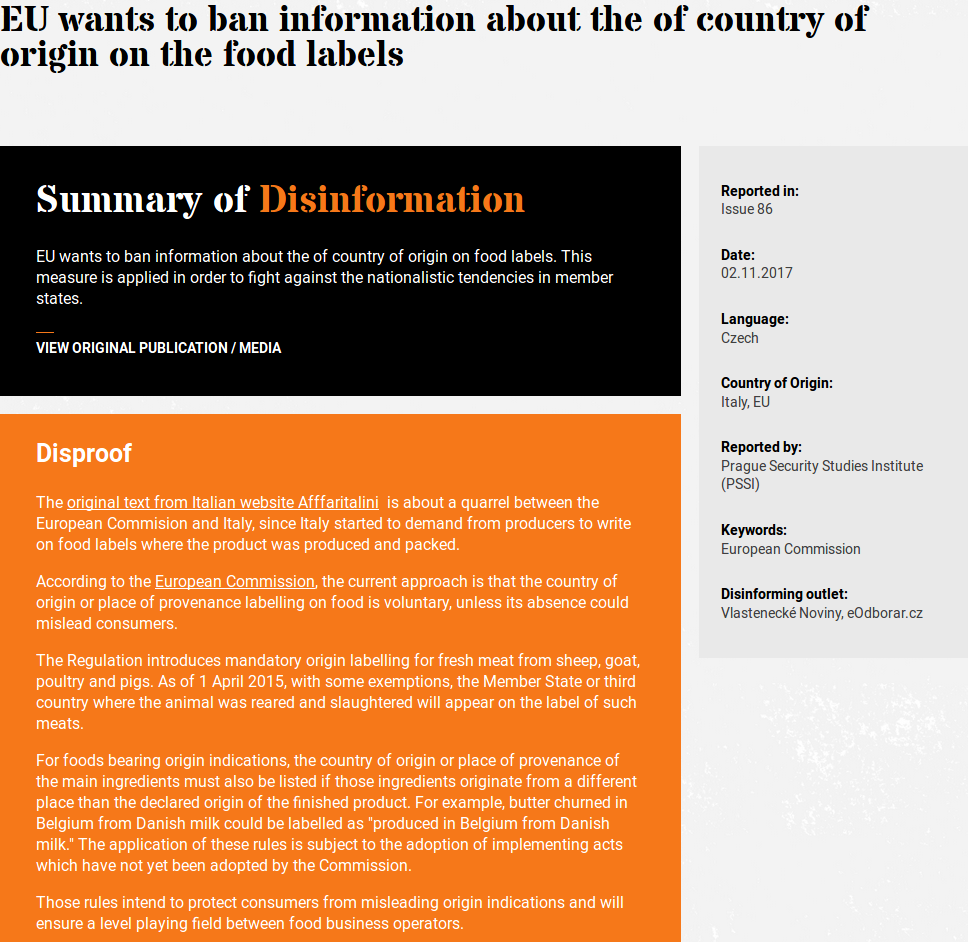
\includegraphics[width=.9\textwidth]{images/example_fakenews.png}
    % \end{subfigure}%
\end{figure}
There is no API, or otherwise download button on the campaign website to get the whole dataset as is. However, there is no mention in their {\texttt robots.txt} file that indicates that scraping is not permitted. Therefore, the intial dataset was achieved after writing a scraper in Python\footnote{\url{https://github.itu.dk/jeshe/fakenews-scraper/blob/master/news_scraper.py}}. The list of cases is an overview list with a pagination of $10$ cases per page, an example of this list is shown in \Cref{fig:cases}. The offset is given by the URL, and so the crawling to acquire links to each specific page can be done in a well defined way, without having to worry about the specific structure of the website.
However, parsing of the structure of the website is necessary in order to scrape the information of each specific case. For this, the python library {\texttt BeautifulSoup}\footnote{\url{https://www.crummy.com/software/BeautifulSoup/}} was heavily used.\\
In the end, the information was saved into a csv file containing one disinformation case per row, and in total $3071$ data rows.

\subsection{Article scraping and content extraction}
In order to get more information that was already available for each case at \url{euvsdisinfo}, information from the original source was also included and added to the dataset. This section will describe the approach that was used in order to reliably get information across the many differently structured websites.
\\\\

\begin{figure}[H]
    % \begin{subfigure}[b]{.3\textwidth}
    \centering
    \caption{An example of a debunked news article from a Czech website}
    % \caption{An example of an original article from a Czech website that was debunked as  }
    \label{fig:fake_source}
    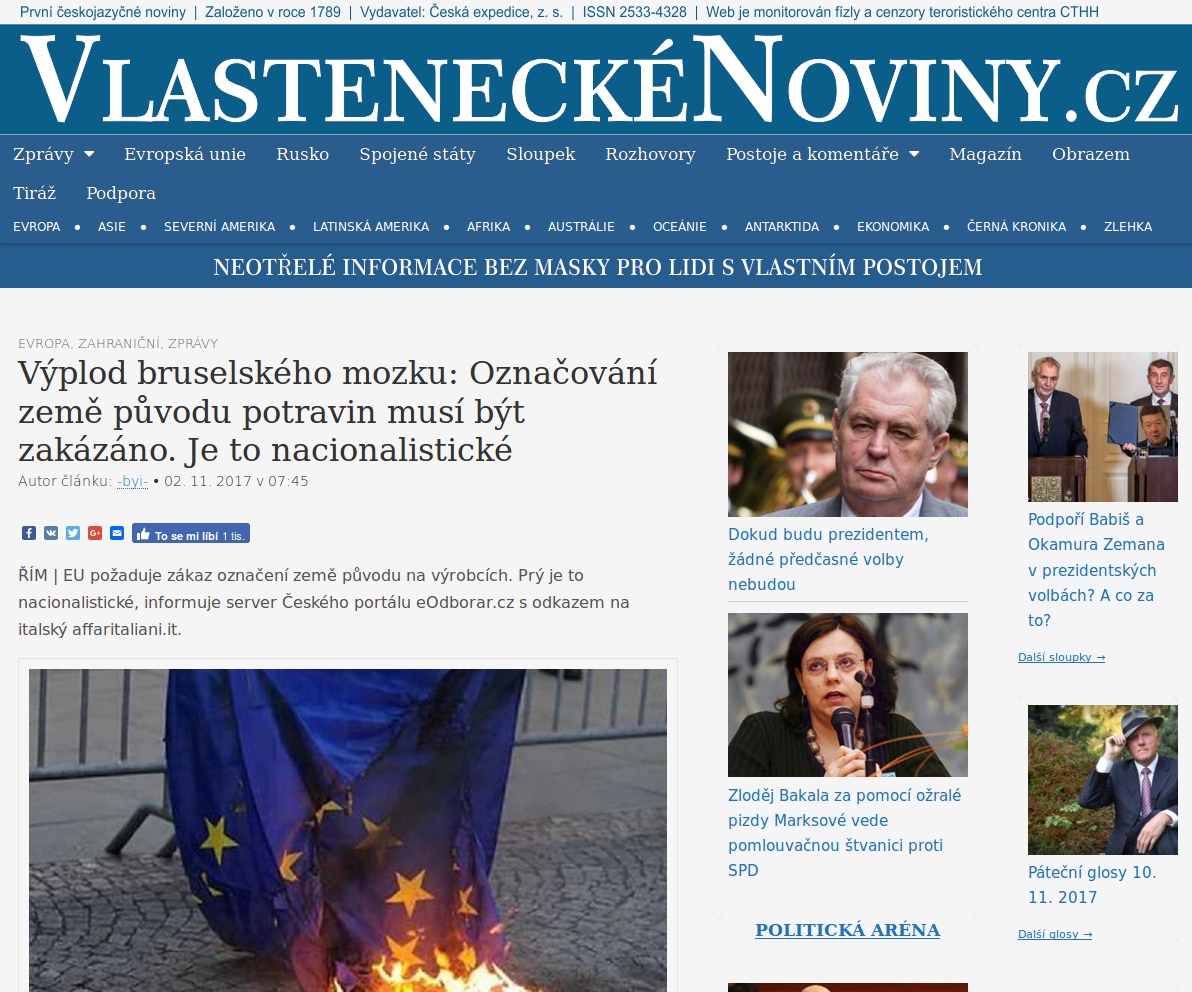
\includegraphics[width=.9\textwidth]{images/example_source.png}
    % \end{subfigure}
\end{figure}
A general approach to extracting content is difficult because source of information can be any sort of media, whether digital or physical, in writing or a video. And, because each website is different, then even building a scraper to extract the content of the subset of sources that are online articles, will be difficult. In \Cref{fig:fake_source} is seen an example of a source article.
\\
One important property for the purpose of this project is that in order to consider the names of locations that are being mentioned in the articles, the entire content is not necessary. Therefore, I chose to use the meta tags to extract information about the content, summary, titles, author, and descriptions of each online resource.
I would also filter on html tags such as the header tags, h1, h2, h3, h4, h5, h6 as well as the title tag used for setting the window title. I found through experiment that only considering the first found header tag worked best, the reason is that other header tags than the first one would often be titles of other news articles that the news site wants the user to click on.
% \\\\
\begin{figure}[H]
\caption{Meta tags defined in python scraper}
\label{fig:python_metatags}
\begin{python}
metatag_list = [
    ("name", "description", "content"),
    ("property" "og:title", "content"),
    ("property", "og:description", "content"),
    ("name", "twitter:title", "content"),
    ("name", "twitter:description", "content"),
    ("name", "language", "content"),
    ("name", "keywords", "content"),
    ("name", "subject", "content"),
    ("name", "topic", "content"),
    ("name", "summary", "content"),
    ("name", "subtitle", "content"),
    ("itemprop", "name", "content"),
    ("itemprop", "description", "content"),
]
tag_list = [ ("h%s" % i, None) for i in range(1, 7) ] + [("title", None)]
\end{python}
\end{figure}

Extracting content by meta tags proved to be a very reliable approach, since most news sites are interested in their content being shared. So, in order to optimize sharability almost all online resources had optimized for search engines, often reffered as just: {\it SEO}. In \Cref{fig:python_metatags} is seen the defined metatags that the scraper was looking for, defined in the variable: {\texttt metatag\_list}, as well as the list of header and title tags defined in {\texttt tag\_list}. Each metatag is defined as a tripplet. The first value defines what attribute to look for when finding a HTML tag of type {\texttt meta}, the second what value such attribute should have. When a match is found for the first two, then the third string in the tripple is used to know from what attribute to extract text from. In the metatags listed in \Cref{fig:python_metatags} all content was extracted from attributes of the same name regardless of the match on the first two. However, defining triples makes this method generalize to any other metatags that might be relevant to add in the future. The reasoning behind the list of other HTML tags being defined as tuples, is similar. Although, for my purposes, the second string was set to {\texttt None}, in which case the script would scrape the inner HTML of the element instead of the content of a named attribute.
\\\\
In order to avoid duplicating content as much as possible the content of a meta tag or html tag was compared to the content that was already found in previous tags. This approach resulted most often in a short paragraph of information about the article, including keywords, title and summary. Before applying the approach to the articles scraped from \href{https://www.euvsdisinfo.eu}{euvsdisinfo.eu}, it was tested on arbitrarily chosen articles, such as articles from danish news outlets. It was also tried on a sample of articles taken from the subreddits: r/politics, r/news, and {r/worldnews}\footnote{\url{https://reddit.com/r/politics+news+worldnews}}, because these were collections of news articles with a good variety of news outlets. The results were used to evaluate qualitatively on the smaller sample. None of which turned out to have no content, and only one resulted in an extract only consisting of keywords. Interestingly, among the keywords for that particular result were also the name of the country that the news story revolved around. \\
One thing that was clear from this, was that locations were not always mentioned if the news concerned well known state leaders such as Putin, Merkel or Trump. In such cases, often only the names of the state leaders were present as indication of what countries were mentioned in the articles.

\subsection{Named entity recognition}
One initially desired outcome was the possibility to extract location information about what countries were being mentioned in the articles. This section will describe the approach to using stanford NER tagger to quantitatively extract location names from the meta information acquired for each article.
\\\\
Named entity recognition is a research field within natural language processing concerned with recognizing names of things such as people, company names, or, as relevant for this project, locations. The study of recognizing location names within texts is one of the most studied areas of named entity recognition, however, still an ongoing research. As such the NER tagger used in this project is released open source as part of the Stanford nlp library\cite{manning-EtAl:2014:P14-5} which also includes many other models and methods relevant to the field of natural language processing. 
%The NER tagger used for this project was a pretrained model trained on a corpus of both e [motherfucking reference] 
A more in depth explanation of named entity recognition or even natural language processing, is however, beyond the scope of this project. 
%Instead for the purposes of this project, I will rely on existing tools.
In \Cref{fig:ner_tagging} is seen an example of tagging a sentence using the graphical interface of the NER tagger. The sentence in \Cref{fig:ner_tagging} is arbitrarily chosen from Wikipedia, and is not part of the content of the dataset.

\begin{figure}[H]
\caption{NER tagging on a sample sentence}
\label{fig:ner_tagging}
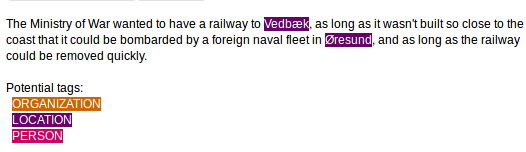
\includegraphics[width=\textwidth]{images/sample_tagging.png}
\end{figure}

The input that was given to the NER tagger was the concatenation of title, summary (as provided by \url{euvsdisinfo}), keywords, and the meta tags content scraped from each individual site.

\subsection{Facebook likes}
The initial dataset, provides only a uniformly weighted list of debunked news cases. In order to provide different weights to the articles in any future visualization, each source URL in the dataset was looked up via facebooks open graph API. The result of the API lookup was a mapping for each source article to a number of likes on facebook, in the case that the information was ever shared on facebook. In \Cref{fig:fetch_likes} is seen the essential part of the python code used for fetching the number of likes of each url. The function {\texttt get\_shares} takes as argument a url and returns dictionary of the response from Facebook's API.

\begin{figure}[H]
\caption{Fetching facebook likes for each source URL}
\label{fig:fetch_likes}
\begin{python}
def get_shares(url):
    enc_url = encode(url)
    access_token = get_access_token()
    fields = "og_object{engagement}"
    api_endpoint = "https://graph.facebook.com/v2.11/%s?fields=%s&access_token=%s"
    return requests.get(api_endpoint % (enc_url, fields, access_token)).json()
\end{python}
\end{figure}

\section{Results}
% The resulting dataset from the previous section consists of the following columns
The resulting dataset from the previous section includes $17$ columns as can be seen in \Cref{tab:resulting_dataset}.
\begin{table}[H]
\caption{Resulting columns in the dataset}
\label{tab:resulting_dataset}
\begin{tabularx}{\textwidth}{| l | X |}
    \hline
    {\bf Column name} & {\bf Description} \\ \hline
    {\texttt issue} & The issue number as given by \href{https://www.euvsdisinfo.eu}{euvsdisinfo.eu}.\\ \hline 
    {\texttt date} & The date the case was reported.\\ \hline
    {\texttt outlet} & The outlet that published the information.\\ \hline
    {\texttt language} & The language the information is provided in.\\ \hline
    {\texttt origin} & Origin of the story, this is sometimes a satirical piece from a different country.\\ \hline
    {\texttt reported by} & The person or organisation who reported the case.\\ \hline
    {\texttt keywords} & Keywords describing the published piece of information.\\ \hline
    {\texttt source} & The URL to the original story, this is not always present i.e. if the source is an interview.\\ \hline
    {\texttt title} & The title of the debunked information.\\ \hline
    {\texttt summary} & The summary of the information that was debunked.\\ \hline
    {\texttt disproof} & The reasoning for \url{euvsdisinfo} to flag the information as dishonest.\\ \hline
    {\texttt metatags} & The types of metatags that included information from the original source during scraping.\\ \hline
    {\texttt metatags\_content} & The content of the metatags that was scraped from the original source.\\ \hline
    {\texttt locations} & Any locations found by the NER tagger.\\ \hline
    {\texttt misc} & Miscellaneously tagged words or phrases tagged by the Stanford NER model. \\ \hline
    {\texttt people} & Recognized names of people by the NER tagger.\\ \hline
    {\texttt likes} & Number of facebook likes registered to the source URL, if any.\\ \hline
\end{tabularx}
\end{table}

The last $6$ columns of \Cref{tab:resulting_dataset} are additions to the initial dataset acquired from \href{https://www.euvsdisinfo.eu}{euvsdisinfo.eu}, namely: {\texttt metatags}, {\texttt metatags\_content}, {\texttt locations}, {\texttt misc}, {\texttt people}, and {\texttt likes}.\\
The most mentioned location is, expectedly, Ukraine. Equally unsurprising is the most frequent language, russian, given the focus of the task force behind the campaign on pro-Kremlin news. The top 5 mentioned locations and the 5 most frequent languages is seen in \Cref{tab:top5}.

\begin{figure}[H]
\caption{5 most frequent languages and top 5 mentioned locations}
\label{tab:top5}
\centering
\begin{tabular}{l | l}
        \begin{tabular}{l | l}
        {\bf language} & {\bf \% of articles} \\ \hline
            Russian     &   55 \\
            Czech       &   16 \\
            English     &   9 \\
            Slovak      &   2 \\
            Georgian    &   2 \\
        \end{tabular} &
        \begin{tabular}{l | l }
        {\bf location} & {\bf \% of articles} \\ \hline
            Ukraine &   27 \\
            Russia  &   23 \\
            USA     &   21 \\
            Europe  &   8  \\
            Syria   &   5  \\ 
        \end{tabular} \\
    \end{tabular}
\end{figure}

In general the NER tagger performed well, only $426$ of the $3071$ cases did not have any locations tagged. A sample of the articles tagged is shown in \Cref{fig:article_title_lang_loc}. The articles shown were chosen based on having the shortest titles in the dataset, simply because they would be easilier presented. As can be seen from \Cref{fig:article_title_lang_loc}, most sources have recognizable locations which seems intuitively correct given the title. However, at least one in these samples, have falsely tagged locations such as {\texttt PravdaReport}, and the word {\texttt Having}. Since measuring such false positives and equally false negatives, cannot be done quantitatively, this inspection has only been done manually on similar samples. However, it is safe to say that the tagged locations cannot be taken for granted as there will be noise in terms of falsely tagged locations. With that in mind, it can serve as a way of depicting the general pattern of locations named in the disinformation sources.

\begin{figure}[H]
\caption{Sample of cases shown by their title, language and locations}
\label{fig:article_title_lang_loc}
\begin{tabular}{l | l | l }
        {\bf title } & {\bf language } & {\bf locations }\\ \hline
        % Russia never met with the AfD & Russian & Russia \\
        Crimea decided its own fate & Russian & Crimea,Russia,China,India \\
        Ukraine is a neo-Nazi state & Russian & Ukraine,West \\
        NATO is encircling Russia. & Czech & Russia \\
        Ukraine is governed by Nazis. & Russian & Ukraine \\
        Sweden wants to leave the EU. & Spain & Sweden \\
        Georgia is a US colony. & Georgian & Georgia,US \\
        Ukraine has a Nazi identity. & Russian & Ukraine \\
        Ukraine is a part of Russia. & Russian & Ukraine,Russia \\
        Savchenko is a US spy. & Russian & US \\
        Nazis control Ukraine. & Russian & Ukraine \\
        NATO kills Serbian children. & English & PravdaReport,West,Russia,Having,\\
                                     &         & Syria,russia,Serbia,Yugoslavia \\
        Ukraine is governed by nazis. & Russian & Ukraine \\
        All Ukraine is Russia. & Russian & Ukraine,Russia \\
    \end{tabular}
\end{figure}

Another interesting aspect appears when looking at the values in the {\texttt reported by} column. More than $\frac{1}{3}$ of the cases has been reported by either of two journalists: Pavel Spirin (780 cases) and Oleksandr Nykonorov (379 cases). In third is the European think-tank \href{http://europeanvalues.net/kremlinwatch}{European Values}. Disregarding possible duplicates in the naming of reporting providers, only 33 entities have reported more than 10 cases out of 193 unique entity names. This is an important aspect to consider, besides the focus of the campaign, when looking at any skewness in the dataset. Oleksandr Nykonorov appears to be a Ukrainian journalist, while the European Values think-tank is an NGO based in the Czech Republic.
\\\\
For the purpose of doing a more visual inspection of the dataset, an online visualization was created using \href{https://d3js.org}{d3}. The visualization uses either of 3 predefined columns from the dataset: {\texttt Language}, {\texttt reported by}, and {\texttt outlet} to create a treemap visualization. While the treemap may not be optimal for all purposes, it goes a long way of showing the above mentioned proportionality within the dataset. In \Cref{fig:viz4kidz} is seen a screenshot of this visualization, the screenshot shows the treemap of the number of articles reported by each person or organization within the different languages. The labels are hard to capture, since, for visual clarity, only entities having reported more than 50 articles have a label. The other will show a label upon mouse hovering. The colors represents different languages, the dark blue, which is most present, represents russian. Each square represents how many articles an entity has reported. As an example it can be seen that for russian, Pavel Spirin has reported the most cases. 

\begin{figure}[H]
\caption{Screenshot of the treemap visualization using grouped data by {\texttt language} and then {\texttt reported by} column}
\label{fig:viz4kidz}
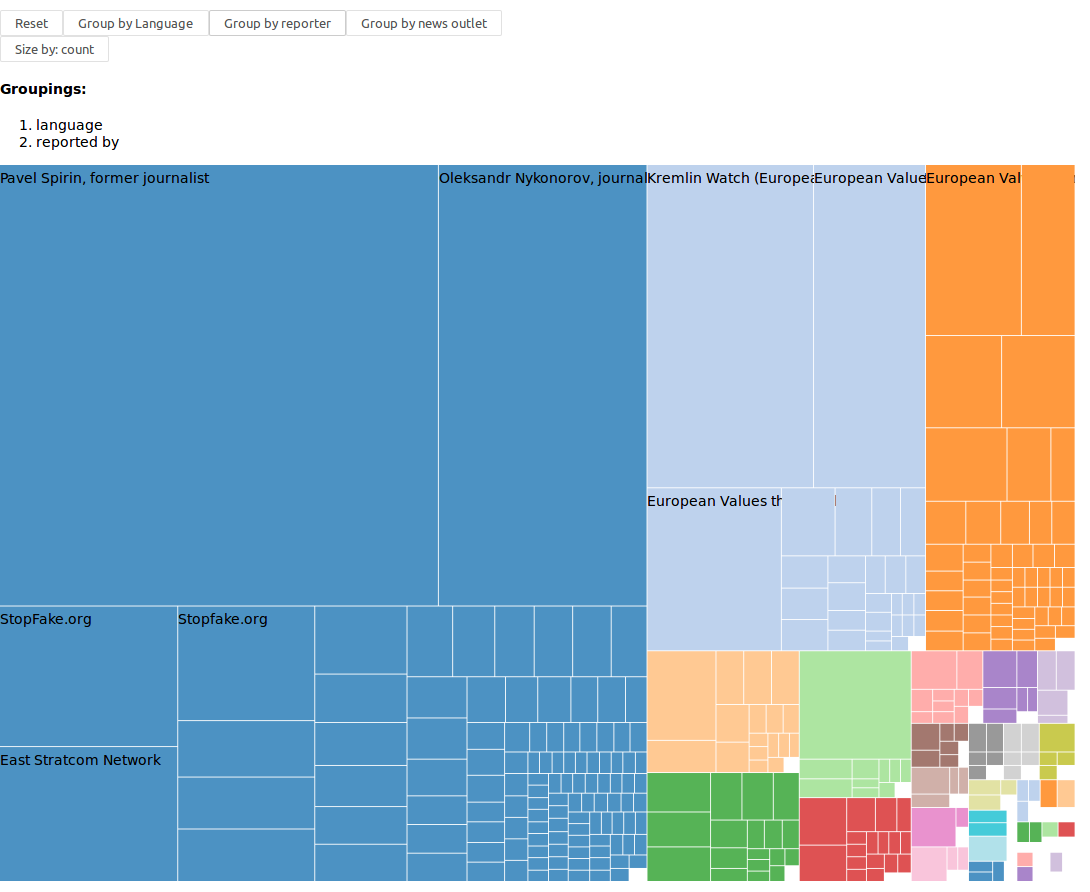
\includegraphics[width=\textwidth]{images/reportedBy_perLanguage_sizeByCount.png}
\end{figure}

Another possible option for the user is to set the size of the squares not by number of cases, but after how many facebook likes each source url accumulated. For information that has not been shared on facebook, the number of likes defaults to zero. The visualization is available as a proof-of-concept at \\\url{http://k4lk.dk:3000}.


\section{Discussion}
% In terms of visualization there are many possibilities, however, perhaps just as many limitations. One such limitation is in regards of an initial vague
Visualizations are difficult as they easily become misrepresentative of the dataset, this is especially true for the domain of fakenews. One example is to consider the cases as attacks by a perpetrator on another vicim, where the roles could be countries or news outlets. However, even as the news outlets, the perpetrator, is provided as part of the data from \href{https://euvsdisinfo}{euvsdisinfo.eu}, then it is hard to automize the extraction of what country is the victim. Often it will be seemingly obvious who the victim is, based on the location and the title or summary of the information. An example of such is russian articles that mentions Ukraine while the NER tagger has recognized the two people mentioned: Adolf Hitler and Petro Poroshenko. \\
However, more often it will be a russian article mentioning two locations: Russia and Ukraine. In such a case it is much more difficult to automize a ruleset of what mentioned country is the actual victim. The reason is that no context is given as to how the locations are being mentioned, so even if an article mentions Russia in a very different light than how it mentions Ukraine, then that context is lost when only the location is extracted, and through a visualization based on this information, both will look like the victim.
\\\\
Furthermore, the dataset itself introduces a lot of biases that if not handled carefully might itself promote a false view of the world to the reader. The fact that the \href{https://euvsdisinfo.eu}{euvsdisinfo.eu} was started in 2015 which correlates with the war in Crimea, and the fact that the campaign already focuses on pro Kremlin news stories, will risk overrepresenting russian news articles. This is especially important if as to not present these data as representative of the state of fake news in the world. The same is true for the campaign itself. When debunking news stories that was never shared on social media in the first place, there is a risk of helping the misinformation more than countering it, simply by giving it publicity that it would never have received otherwise. Even if that publicity is negative, it might be more in the interest of the original outlet than simply not having any attention.
\\\\
That attention is important is stressed by the fact that the majority of news outlets that were online, had optimized for search engines. Their objective to be as shareable as possible, since they will want their information to spread in order to be effective, by definition makes these websites easily available to crawl and scrape in a structured, reliable way. At least as reliable as webscraping goes. 
%Even if the set of articles as a whole, is unstructured, simply because each website is very different.
\\ 
In this project the attempt to extract information about people and locations that were mentioned in the online articles, worked well using the metatags provided for search engines. The lack of context the words appeared in, made it hard to automize any interpreting visualization. However, it is still interesting without a layer of interpretation to be able to look at the distribution of locations as it provides a perspective on how the focus on Russia manifests itself in the dataset.
\\\\
The aspect of disproportionality is also interesting in regards to how these cases are presented on the campaign website. All cases as illustrated in \Cref{fig:cases} is shown with a uniform importance. However, as seen when requesting the likes via the facebook API for each URL, it becomes clear, that the distribution of likes is very different from this uniform presentation. Whether or not likes is a good measure of impact, the perspective is arguably different when sizing the treemap using the likes of each case, instead of just counting each case. The difference is visually inspectable through the online visualization, \url{http://k4lk.dk:3000}. In \Cref{fig:lang_bycountorlikes} is seen a screenshot of each of these two cases. The figures shows the cases grouped by the language they were published in. However, as can be seen in \Cref{subfig:lang_count}, the by far most present language in terms of information cases, is russian, but if the same view is measured in number of likes, seen in \Cref{subfig:lang_likes}, then english accumulates more than double the amount of likes as the second most liked russian languaged sources (light blue). In \Cref{subfig:lang_likes} each square represents an article, thereby it can be seen that a few specific cases dominates in terms of accumulating likes. A few specific cases being exponentially more liked than others, can be seen from the visualization as a pattern across all languages.
% simple sentiment using hitler etc.
% similarly, the combination of title, language, and locations could be interesting:
% the focus on pro-kremlin news together with the Crimea crisis is probably the reason why most mentioned location is Ukraine
% problem making an attack map, since locations are given no context
% structured/unstructured tension

\begin{figure}[H]
\caption{Cases grouped by language and sized either by number of cases, or accumulated likes of the cases}
\label{fig:lang_bycountorlikes}
\begin{subfigure}{\textwidth}
\caption{Language by number of articles}
\label{subfig:lang_count}
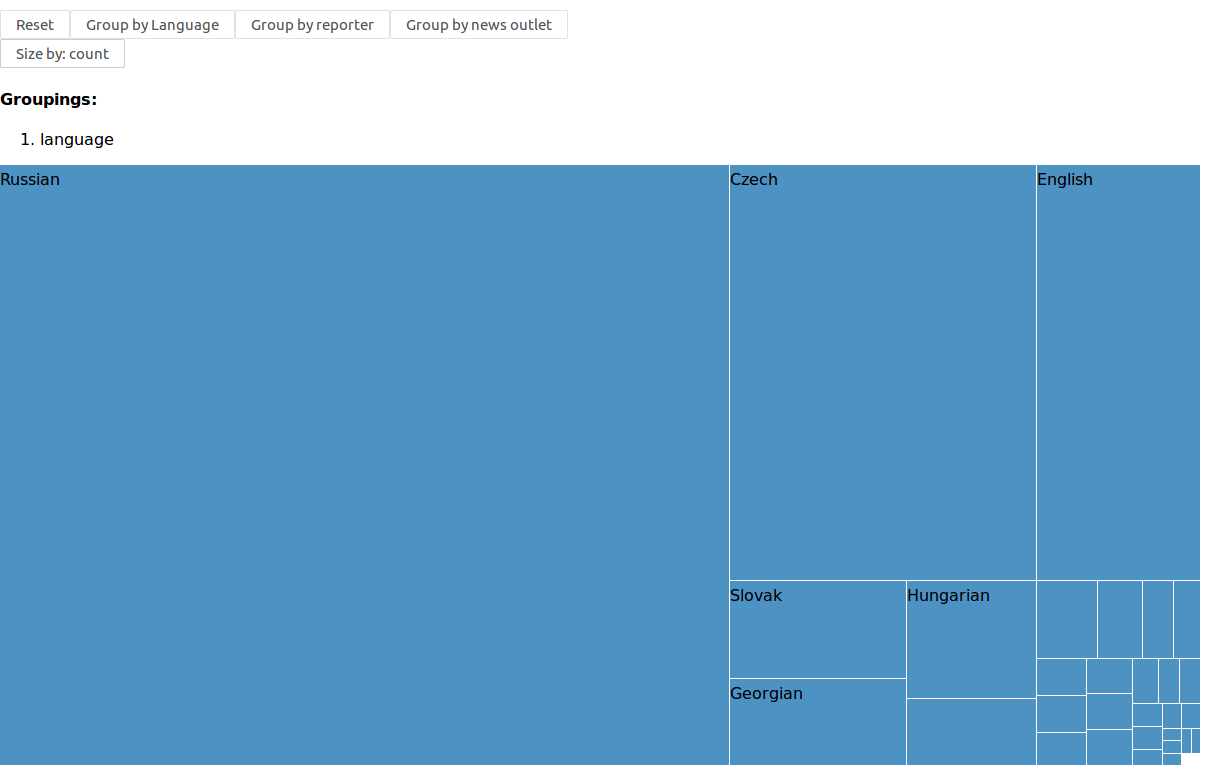
\includegraphics[width=\textwidth]{images/lang_by_count.png}
\end{subfigure}
\begin{subfigure}{\textwidth}
\caption{Language by amount of likes}
\label{subfig:lang_likes}
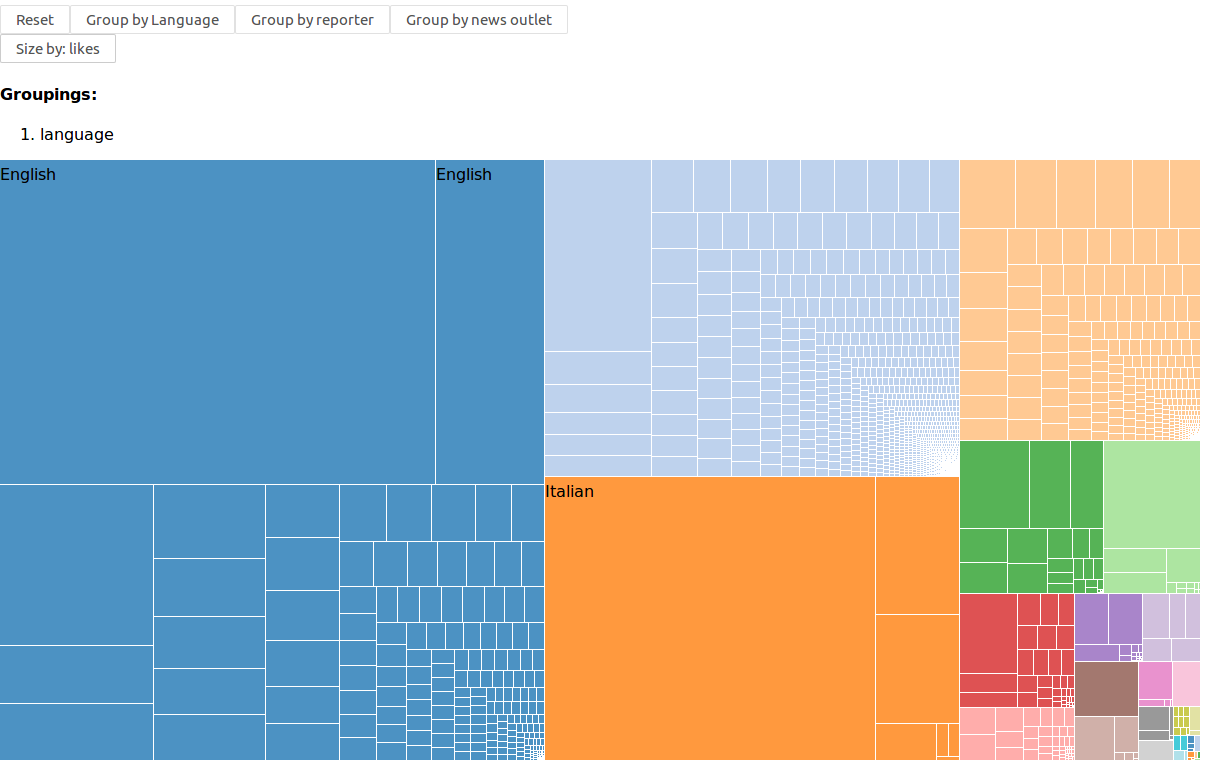
\includegraphics[width=\textwidth]{images/lang_by_likes.png}
\end{subfigure}
\end{figure}

\section{Conclusion}
In order to be able to better counter the impact of fakenews, we need a better understanding of the nature of fakenews. In this project a very small part of the entire body of fakenews were looked at, namely the cases available from \href{https://euvsdisinfo.eu}{euvsdisinfo.eu}.
\\\\
Even though the nature of fake news makes it nearly impossible to automate the visualization or analysis of fake news, it is still possible through semi automatic methods, as illustrated in this report. This is only achievable because of resources such as \href{https://euvsdisinfo.eu}{euvsdisinfo.eu}, that makes the metainformation available as collections in a structured manner. In the same way that the various ways information can be debunked, is not achievable in an automatic way, the same can be said for the deeper interpretations of the eventually debunked cases. However, creating a visual perspective goes a long way to better our understanding of underlying patterns. As is true for many complex phenomenons, then no single perspective can provide the whole truth. Similarly, to visualize the underlying patterns in the dataset used for this project, many different views is needed. For this reason, the explorable visualization is a good approach, however the concrete treemap that was the outcome of this project, can only be seen as a limited part of the perspectives needed to understand the phenomenon of fake news.

\newpage
\bibliographystyle{abbrv}
\bibliography{lit}
\end{document}